%!TEX root = slides2.tex
% Добавьте ссылку на файлы с текстом работы
% Можно использовать команды:
%   \input или \include
% Пример:
%    \input{mainfiles/1-section} или \include{mainfiles/2-section}
% Команда \input позволяет включить текст файла без дополнительной обработки
% Команда \include при включении файла добавляет до него и после него команду
% перехода на новую страницу. Кроме того, она позволяет компилировать каждый файл
% в отдельности, что ускоряет сборку проекта.
% ВАЖНО: команда \include не поддерживает включение файлов, в которых уже содержится команда \include,
% т.е. не возможен рекурсивный вызов \include
\newcommand*{\Source}{
    %!TEX root = ../slides2.tex

\section{Referring object segmentation}

\begin{frame}
  \frametitle{Referring object segmentation}
  \begin{itemize}
    \item \textbf{Referring video object segmentation (R-VOS)} -задача сегментации объекта на видео по его описанию на натуральном языке.
    \item \textbf{Referring image segmentation} - задача сегментации объекта на изображении по его описанию на натуральном языке.
    
  \end{itemize}
\end{frame}


\section{Актуальность}

\begin{frame}
  \frametitle{Актуальность}
  \begin{itemize}
    \item видеонаблюдение 
    \item приложения для редактирования изображений и видео 
    \item обнаружение патологий на медицинских изображениях
    \item взаимодействие человека и робота посредством языка
  \end{itemize}
  
\end{frame}


\section{Цель}
\begin{frame}
    \frametitle{Цель}
    \begin{itemize}
        \item Дан видеоклип \(V=\{I_t\}_{t=1}^{T}\), содержащий \(T\) фреймов и
        текстовое описание сегментируемого объекта из этого клипа: \(E=\{e_l\}_{l=1}^L\), состоящее из \(L\) слов. \\
        Цель: создать маску сегментации описываемого объекта 
        \(S=\{s_t\}_{t=1}^T, s_t \in \mathbb{R}^{HxW}\), для каждого фрейма. 
        \item Дано изображение \(I\) и текстовое описание сегментируемого объекта из этого изображения: \(E=\{e_l\}_{l=1}^L\), состоящее из \(L\) слов. \\Цель: создать маску сегментации описываемого объекта.

    \end{itemize}
\end{frame}

\section{Постановка задачи}
\begin{frame}
  \frametitle{Постановка задачи}
  \begin{itemize}      
    \item Сделать обзор существующих методов сегментации объектов на видео/изображении по текстовому описанию.
    \item Запустить существующие решения.
    \item Рассмотреть идеи по улучшению или обобщению сегментации
    \item Провести эксперименты с применением улучшений
  
\end{itemize}
\end{frame}
    %!TEX root = ../slides2.tex

\section{Language as Queries for RVOS}

\begin{frame}
    \frametitle{Language as Queries for RVOS}
    \begin{figure}
        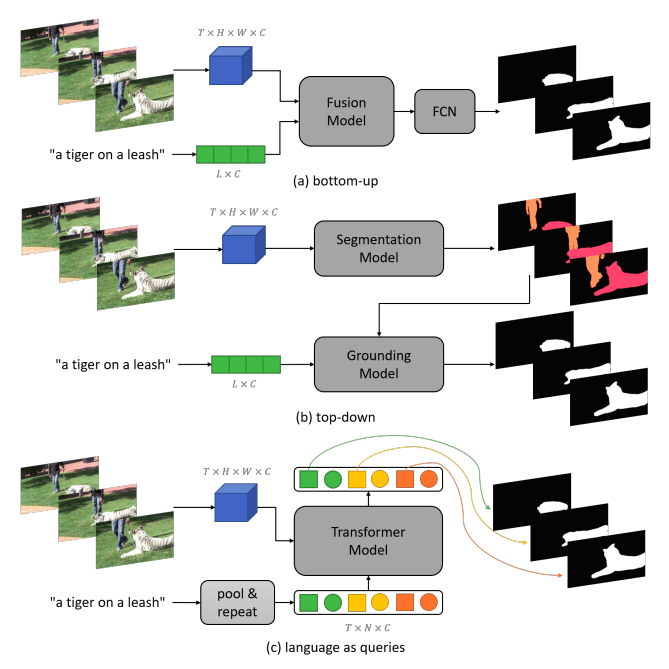
\includegraphics[scale=0.32]{btom.png}
    \end{figure}
\end{frame}

\subsection{Архитектура}

\begin{frame}
    \frametitle{Language as Queries for RVOS. Архитектура}
    \begin{figure}
        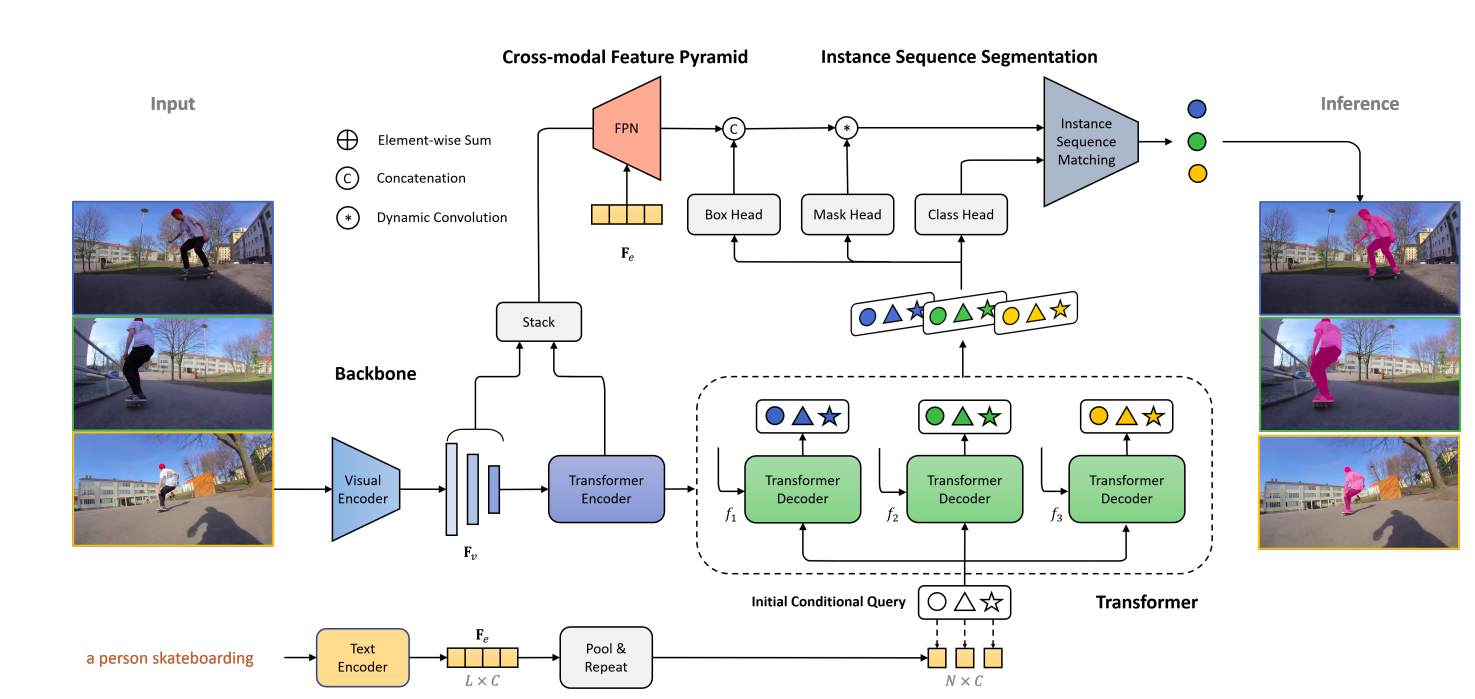
\includegraphics[scale=0.25]{rvosarch.png}
    \end{figure}
\end{frame}
    %!TEX root = ../slides2.tex

\section{Vision-Language Transformer and Query Generation for Referring
Segmentation}
\begin{frame}
    \frametitle{Queries}
    \begin{figure}
        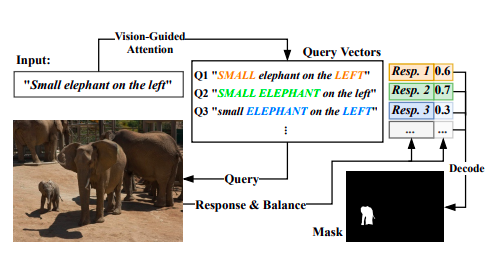
\includegraphics[scale=0.5]{queries.png}
    \end{figure}
\end{frame}
\subsection{Архитектура}
\begin{frame}
    \frametitle{Vision-Language Transformer and Query Generation for Referring
    Segmentation. Архитектура}
    \begin{figure}
        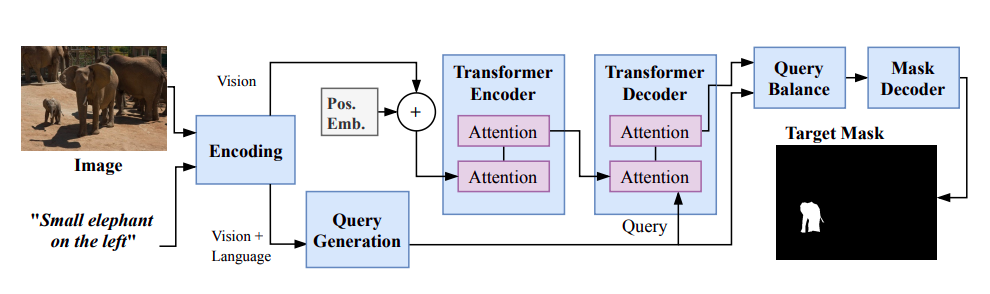
\includegraphics[scale=0.35]{risarch.png}
    \end{figure}
\end{frame}
    %!TEX root = ../slides2.tex

\section{Примеры}
\begin{frame}
    \frametitle{Примеры}
    \begin{itemize}
        \item \textcolor{blue}{\href{https://github.com/wjn922/ReferFormer}{Language as Queries for RVOS}}
        \item \textcolor{blue}{\href{https://github.com/mttr2021/MTTR/tree/c383c5b151e3c97aeb45cd2fb4bf08719016498b}{MTTR}}
        \item \begin{figure}
            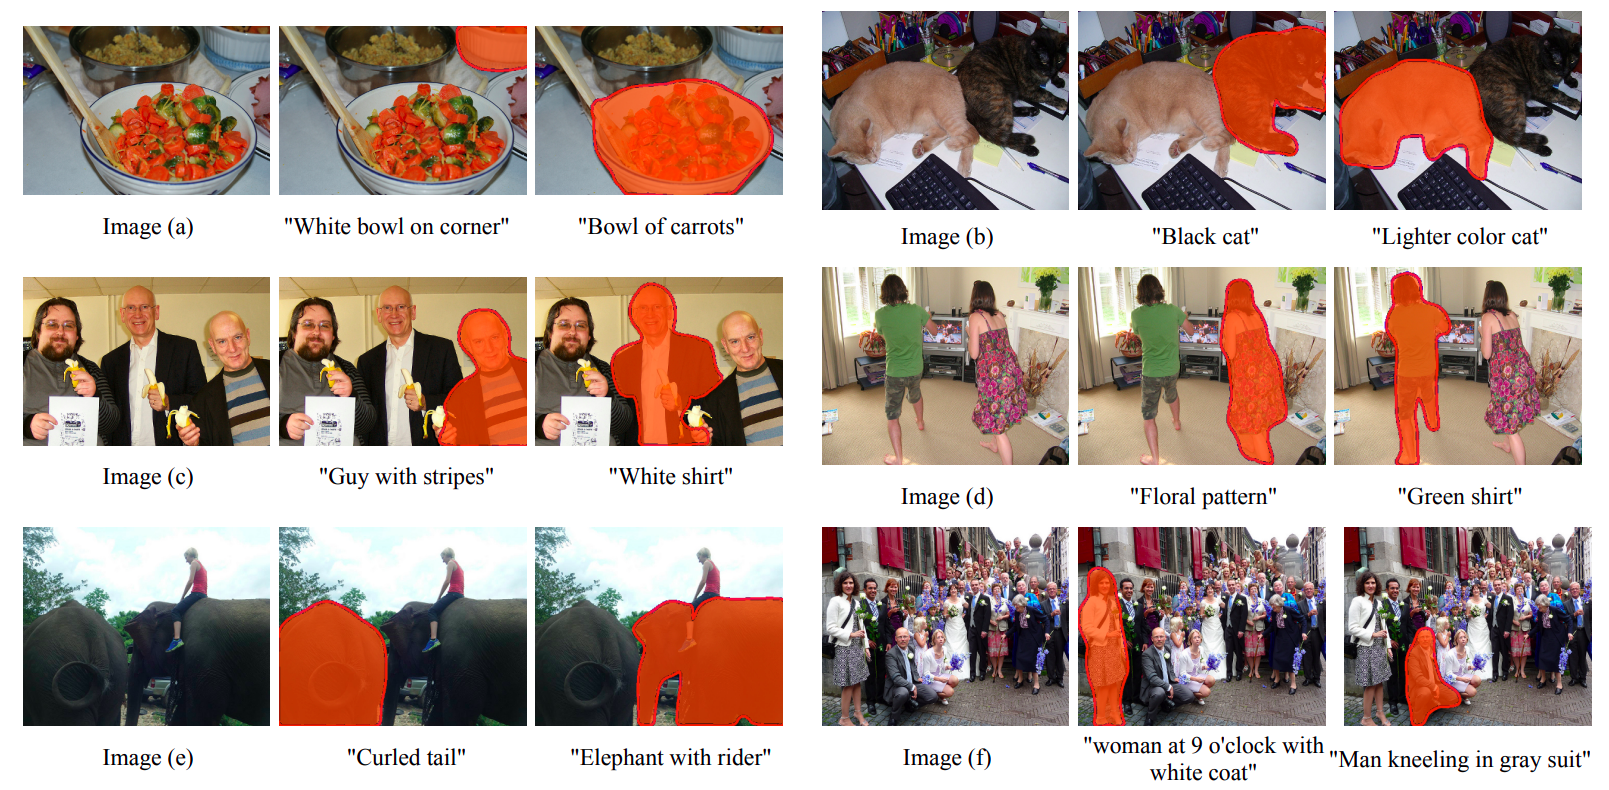
\includegraphics[scale=0.15]{example.png}
        \end{figure}
    \end{itemize}
    
\end{frame}


    %!TEX root = ../slides2.tex
\section{Датасеты}
\begin{frame}
    \frametitle{Датасеты}
    \begin{itemize}
        \item A2D-Sentences: A Dataset and Benchmark for Action Recognition and Segmentation with Multiple Classes of Actors
        \begin{figure}
            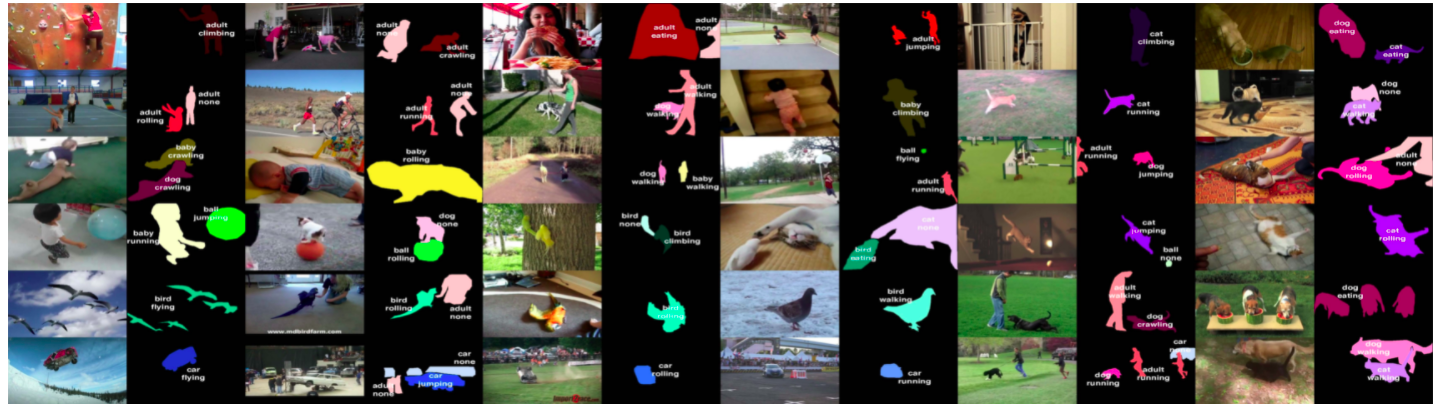
\includegraphics[scale=0.25]{a2d.png}
        \end{figure}
        \item JHMDB-Sentences: A fully annotated data set for human actions and human poses.
        \item Refer-YouTube-VOS
    \end{itemize}
\end{frame}

\section{Loss}
\begin{frame}
    \frametitle{Loss}
    \begin{itemize}
        \item \(\overline{y}=\{\overline{y_i}\}_{i=1}^{N}\)- множество предсказаний
        \item для каждого \(i\)
        предсказание имеет вид: \(\overline{y_i}=\{\overline{p}^t_i,\overline{b}^t_i, \overline{s}^t_i\}_{t=1}^T\)
        \item правильный ответ имеет вид: \(y=\{c^t,b^t,s^t\}_{t=1}^T\) 
        \begin{itemize}
            \item \(\overline{y}_{pos} = \underset{\overline{y_i}\in\overline{y}}{argmin} L_{match}(y, \overline{y_i})\)
            \item \(L_{match}(y, \overline{y_i})=k_{cls}L_{cls}(y, \overline{y_i})+
            k_{box}L_{box}(y, \overline{y_i})+ k_{mask}L_{mask}(y, \overline{y_i})\)
        \end{itemize}
    \end{itemize}
\end{frame}

\section{Метрики}
\subsection{IoU}
\begin{frame}
    \frametitle{Метрики}
    \begin{itemize}
        \item IoU:
         \begin{figure}
            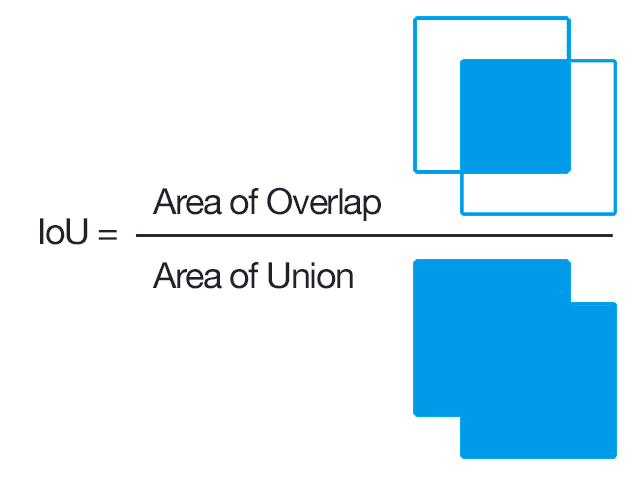
\includegraphics[scale=0.2]{iou.png}
        \end{figure}
        
    \end{itemize}
\end{frame}
\subsection{mAP}
\begin{frame}
    \frametitle{Метрики}
    \begin{itemize}
        \item \(mAP\):
        \begin{itemize}
            \item \(p=\frac{TP}{TP+FP}, \quad r=\frac{TP}{TP+FN}\)
            \item \(AP=\int_{0}^{1}p(r)dr\)
            \item \(mAP=\frac{1}{n}\sum_{i=1}^{n}AP_{i}, n -\)количество классов, \(AP_{i} - AP\) для \(i\)-го класса
        \end{itemize}

        \begin{figure}
            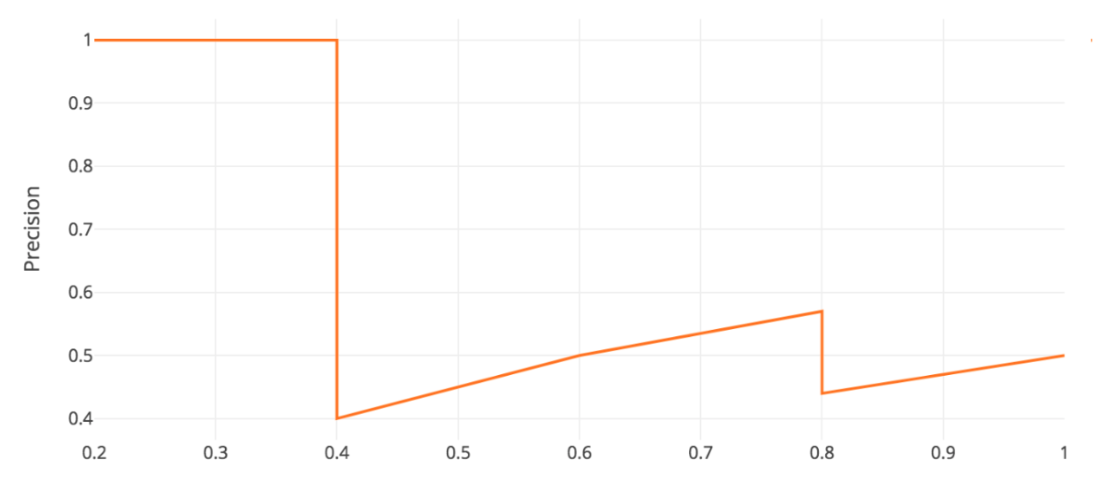
\includegraphics[scale=0.2]{prcurve.png}
        \end{figure}
    \end{itemize}
\end{frame}

\section{План работ}
\begin{frame}
    \frametitle{План работ}
    \begin{itemize}      
        \item Сделать обзор существующих методов сегментации объектов на видео по текстовому описанию - \textbf{сделано}.
        \item Запустить существующие решения - \textbf{сделано}.
        \item Рассмотреть идеи по улучшению или обобщению сегментации (например, bilingual - сегментация)
        \item Провести эксперименты
      
    \end{itemize}
\end{frame}


\begin{frame}
    \begin{center}
        \text{СПАСИБО ЗА ВНИМАНИЕ!}
    \end{center}
\end{frame}
 
}


% Информация о годе выполнения работы
\newcommand{\Date}{%
    % 16 июня 2010 г.%
    \today%     % Текущий день
}

% Укажите тип работы
% Например:
%     Выпускная квалификационная работа,
%     Магистерская диссертация,
%     Курсовая работа, реферат и т.п.
\newcommand{\WorkType}{%
    % Выпускная квалификационная работа%
    % Магистерская диссертация%
     Курсовая работа%
    % Реферат%
    %Дипломная работа%
}

% Название работы
%%%%%%%%%%% ВНИМАНИЕ! %%%%%%%%%%%%%%%%
% В МГУ ОНО ДОЛЖНО В ТОЧНОСТИ
% СООТВЕТСТВОВАТЬ ВЫПИСКЕ ИЗ ПРИКАЗА
% УТОЧНИТЕ НАЗВАНИЕ В УЧЕБНОЙ ЧАСТИ
\newcommand{\Title}{%
    Сегментация объектов на видео и изображениях по текстовому описанию%
}


% Имя автора работы
\newcommand{\Author}{%
    Айрапетьянц Каринэ Арсеновна%
}

% Информация о научном руководителе
%% Фамилия Имя Отчество%
\newcommand{\SciAdvisor}{%
    Малоян Нарек Гагикович%
}
%% В формате: И.~О.~Фамилия%
\newcommand{\SciAdvisorShort}{%
    Н.~Г.~Малоян%
}
%% должность научного руководителя
\newcommand{\Position}{%
    % профессор%
    %доцент%
    % старший преподаватель%
    % преподаватель%
    % ассистент%
    % ведущий научный сотрудник%
    % старший научный сотрудник%
    % научный сотрудник%
    % младший научный сотрудник%
}
%% учёная степень научного руководителя
\newcommand{\AcademicDegree}{%
    % д.ф.-м.н.%
    % д.т.н.%
    %к.ф.-м.н.%
    % к.т.н.%
    % без степени%
}

% Информация об организации, в которой выполнена работа
%% Город
\newcommand{\Place}{%
    Москва%
}
%% Университет
\newcommand{\Univer}{%
    Московский государственный университет имени М.~В.~Ломоносова%
}
\newcommand*{\UniverAbbr}{%
    МГУ%
}
%% Факультет
\newcommand{\Faculty}{%
    Факультет вычислительной математики и кибернетики%
}
%% Кафедра    
\newcommand{\Department}{%
    Кафедра информационной безопасности%
}     

%%%% Переключите формат экрана
\newcommand{\Aspect}{%
    % 43%
    % 1610%
    169%
}
